
The equation of the linear regression line for this data using the 59.541 keV
peak of $^{241}$Am and the  661.657 keV peak from $^{137}$Cs.

\begin{equation}
Energy=0.280576(channel)+1.181092
\end{equation}

This model is then used to calibrate both $^{241}$Am and $^{137}$Cs
data, and is displayed in Figure \ref{fig:fit}.



\begin{figure}[H]
\begin{center}
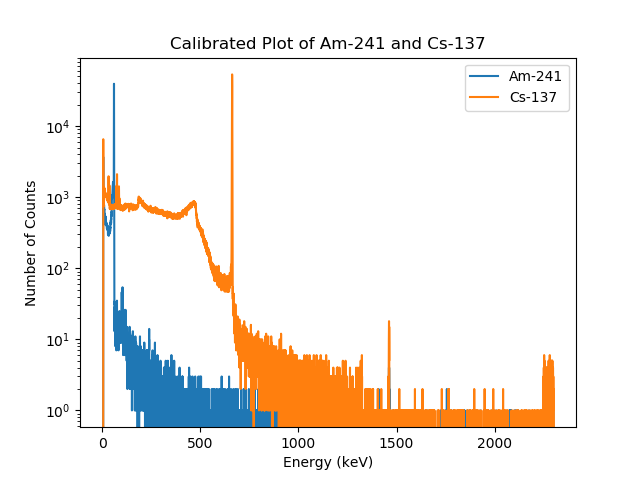
\includegraphics[width=.7\linewidth]{../images/cal_AmCs.png}
\caption{Calibrated Americium and Cesium Spectrum
\label{fig:fit}}
\end{center}

\end{figure}



Comparing the calibrated pulse height spectrum of $^{133}$Ba
to its true values as specified in the nuclear data literature
we find that the model is sufficiently accurate. The full comparison is
displayed in the table below.

\pgfplotstabletypeset[%
   fixed zerofill,
   precision=4,
   col sep=space,
   dec sep align,
   columns/0/.style ={column name=Actual Energy (KeV)},
   columns/1/.style ={column name=Calibrated Energy (KeV)},
   columns/2/.style ={column name=Percent Difference (\%)},
]{./images/peakdiffquant.csv}
